% Bagian latent saja, mengikuti papan tulis dosen: V (embedding), V1 (weak), V2 (strong), dan syarat cosine-nya.
% Angka contoh: V = [3,0,4,0], r = [1,2,0,0]; V1 dan V2 sama dengan di cosine_hitung.tex (c = 0,8 dan 0,4); cosine diperiksa.
% Kompilasi (dari folder ini): pdflatex cosine_latent.tex && pdftoppm -png -r 300 -singlefile cosine_latent.pdf cosine_latent
\documentclass[border=6pt]{standalone}
\usepackage{amsmath}
\usepackage{amssymb}
\usepackage{mathptmx}
\usepackage{tikz}
\usetikzlibrary{arrows.meta, calc}

\definecolor{ink}{HTML}{3A3936}
\definecolor{muted}{HTML}{8A8984}
\definecolor{modelE}{HTML}{2A78D6}
\definecolor{augE}{HTML}{EB6834}

\tikzset{
  every node/.style={font=\normalsize, text=ink, align=center},
  flow/.style={-{Stealth[length=3mm]}, line width=1.3pt, draw=ink, rounded corners=5pt},
  tag/.style={font=\footnotesize\itshape, text=muted},
}

\begin{document}
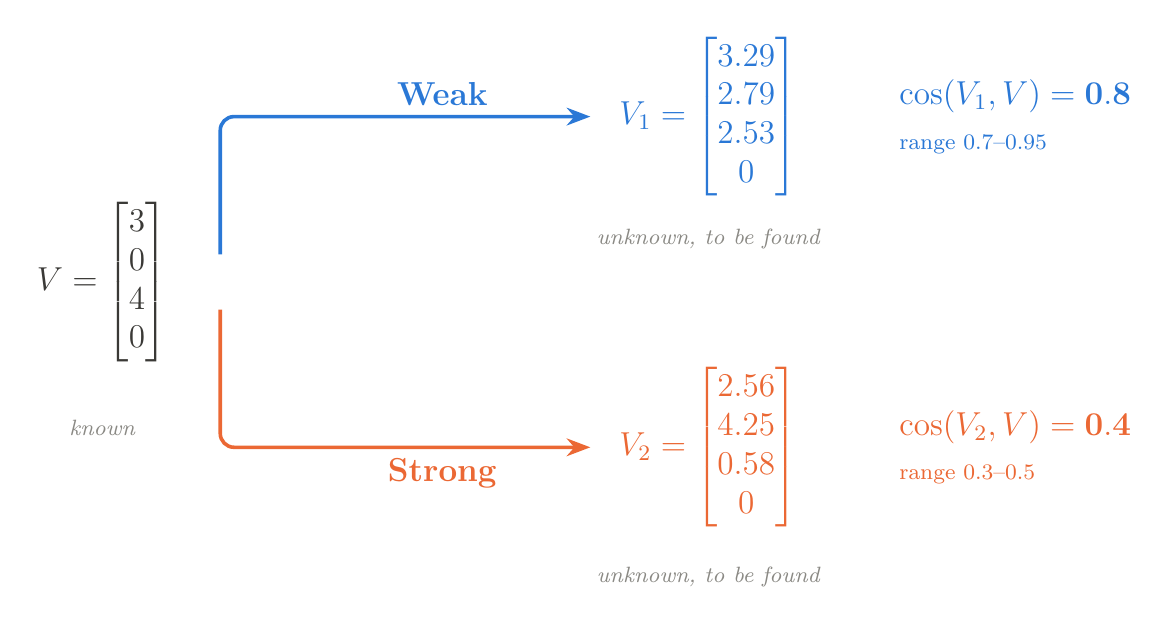
\begin{tikzpicture}

% V (embedding asli)
\node[font=\large] at (0,0) {$V=\begin{bmatrix}3\\0\\4\\0\end{bmatrix}$};
\node[tag] at (0,-1.85) {known};

% cabang weak dan strong
\draw[flow, modelE] (1.5,0.35) |- node[pos=0.8, above, text=modelE, font=\large\bfseries] {Weak} (6.2,2.1);
\draw[flow, augE]   (1.5,-0.35) |- node[pos=0.8, below, text=augE, font=\large\bfseries] {Strong} (6.2,-2.1);

% V1 (weak)
\node[font=\large, text=modelE] at (7.7,2.1) {$V_1=\begin{bmatrix}3.29\\2.79\\2.53\\0\end{bmatrix}$};
\node[font=\large, text=modelE, anchor=west, align=left] at (10.0,2.1) {$\cos(V_1,V)=\mathbf{0.8}$\\[2pt]\footnotesize range $0.7$--$0.95$};
\node[tag] at (7.7,0.55) {unknown, to be found};

% V2 (strong)
\node[font=\large, text=augE] at (7.7,-2.1) {$V_2=\begin{bmatrix}2.56\\4.25\\0.58\\0\end{bmatrix}$};
\node[font=\large, text=augE, anchor=west, align=left] at (10.0,-2.1) {$\cos(V_2,V)=\mathbf{0.4}$\\[2pt]\footnotesize range $0.3$--$0.5$};
\node[tag] at (7.7,-3.75) {unknown, to be found};

\end{tikzpicture}
\end{document}
